% Chapter Template

\chapter{Medologías y Herramientas de Trabajo} % Main chapter title
% cSpell:words resizebox \textit{onosapi} usecase Mcast enrutamiento parencite includegraphics pcktprocactiv lstlisting iperf

\label{Chapter5} % Change X to a consecutive number; for referencing this chapter elsewhere, use 
% \ref{ChapterX} 
En la actualidad, existen diversas metodologías para el desarrollo del software separadas en dos grandes grupos: metodologías tradicionales y metodologías ágiles. 

Será importante definir y adoptar alguna de ellas con el fin de establecer convenciones para el desarrollo del proyecto integrador. Se aborda así en la primer sección de este capítulo, la metodología de trabajo utilizada en las diferentes etapas.

Luego, se definen las herramientas de trabajo empleadas durante el desarrollo del proyecto y finalmente se describe la planificación de riesgos.

%----------------------------------------------------------------------------------------
%	SECTION 1
%----------------------------------------------------------------------------------------

\section{Metodología de desarrollo de software}
Para la gestión del desarrollo del software de este proyecto, se utilizó la metodología ágil iterativa e incremental. Dicha metodología consiste en dividir el proyecto en iteraciones bien definidas. En cada una de estas iteraciones se agregan nuevas funcionalidades y también se pueden introducir mejoras sobre las iteraciones anteriores. Los factores determinantes para la decisión de esta metodología se listan a continuación:

\begin{itemize}
	\item Existe la necesidad de tener una metodología en la cual se realicen reportes al director y co-director del proyecto, quienes analizarán los avances.
	\item Al dividir el proyecto en etapas, permite centrar la atención y organización a una pequeña parte de la misma.
	\item La necesidad de tener una metodología que sea flexible ante requerimientos cambiantes.
\end{itemize}
%-----------------------------------
%	SUBSECTION 1
%-----------------------------------

\subsection{Organización de las iteraciones}
Una vez definida la metodología para la gestión del proyecto, se definieron en conjunto con el director y co-director las iteraciones que conformarán el proyecto. Las mismas se presentan a continuación.
\begin{itemize}
	\item \textbf{Iteración 1: Familiarización con el \textit{muxponder}.} El objetivo de esta iteración es entender cómo funciona el equipo, sus capacidades, aplicaciones y utilidades.
	\item \textbf{Iteración 2: Investigación del protocolo \textit{NETCONF}.} Esta iteración tiene como objetivo realizar un estudio sobre el protocolo \textit{NETCONF}, las distintas implementaciones disponibles y cómo utilizar las mismas.
	\item \textbf{Iteración 3: Adaptación del agente \textit{NETCONF} al \textit{muxponder}.} Esta etapa del proyecto consiste en adaptar algún agente al equipo, realizando pruebas sobre las funcionalidades, capacidades y limitaciones del mismo.
	\item \textbf{Iteración 4: Realización de la librería en el \textit{muxponder}.} Independientemente del agente utilizado en el equipo, se deberá realizar una aplicación que relacione el agente \textit{NETCONF} con la instrumentación del \textit{muxponder}.
	\item \textbf{Iteración 5: Desarrollo del \textit{driver} en el controlador.} El objetivo de esta iteración será la de realizar un \textit{driver} en el controlador para que el mismo pueda comunicarse con los diferentes \textit{muxponders} presentes en la topología.
	\item \textbf{Iteración 6: Realización de la aplicación API REST en el controlador.} En esta etapa, se desarrolla la aplicación \textit{REST} que expone las distintas funcionalidades implementadas en el \textit{driver} del controlador, para que aplicaciones externas puedan hacer uso del mismo.
	\item \textbf{Iteración 7: Desarrollo de la interfaz gráfica.} Finalmente en esta iteración se desarrolla la interfaz gráfica, la cual a través de la API REST desarrollada, se comunica con los diferentes equipos haciendo uso del controlador y las bondades de \textit{SDN}.
\end{itemize}

\section{Lenguajes de programación}
En el presente trabajo de fin de grado, se utilizaron diversos lenguajes de programación. Se presenta a continuación una lista de los lenguajes empleados como así también la etapa en la cual fueron aplicados. 

\begin{itemize}
	\item \textbf{C}. El agente Yuma123 y la librería en C que comunica la instrumentación del dispositivo con el agente, se encuentran desarrollados en dicho lenguaje.  
	\item \textbf{Java}. Tanto el controlador \textit{ONOS}, como el \textit{driver} y la \textit{API REST} que se desarrolló, se encuentran escritos en dicho lenguaje. 
	\item \textbf{Python}. Durante el diseño de la interfaz gráfica, se optó por \textit{Flask} como \textit{web server}, el cual consiste en un \textit{framework} minimalista escrito en \textit{Python} que permite crear aplicaciones \textit{web} de forma rápida y sencilla. 
\end{itemize}

\section{Herramientas de desarrollo}
Las herramientas que conforman el entorno de desarrollo se listan a continuación.

\begin{itemize}
	\item \textbf{IntelliJ IDEA} como entorno de desarrollo utilizado para proyectos \textit{Java} y \textit{Python}.  
	\item \textbf{Mavenen} para la gestión de proyectos \textit{Java}, empleado especificamente en la construcción del controlador \textit{ONOS}.
	\item \textbf{Visual Studio Code} como editor de código fuente, utilizado en multiples etapas del proyecto.
\end{itemize}

\section{Control de versiones}
Se optó por utilizar el sistema de control de versiones conocido como \textit{Git} \parencite{gitref} alojado en un servidor de \textit{GitHub} \parencite{githubref}. El hecho de utilizar un sistema de control de versiones supone las siguientes ventajas:

\begin{itemize}
	\item Mantiene un historial de versiones del software. De esta forma, cada cambio se encuentra versionado permitiendo que en cualquier momento se pueda regresar el código a estados anteriores o comparar los cambios entre las distintas versiones del mismo.   
	\item Acceso remoto al proyecto. Al utilizar un servidor de \textit{Git} público, el proyecto puede ser accedido de forma remota desde cualquier equipo para continuar con el desarrollo del mismo en cualquier momento.
	\item Utilización de un esquema de ramas. Permite trabajar de manera paralela sobre diferentes partes del proyecto sin interferencias, permitiendo integrar nuevas funcionalidades al software de manera segura.
\end{itemize}

\section{Planificación de riesgos}
Todo desarrollo de software implica una serie de riesgos e incertidumbres que deben ser planificadas para definir una forma estructurada de actuar ante ellas, con el fin de cumplir con los tiempos establecidos.

El objetivo es identificar y analizar los riesgos que se puedan presentar para establecer estrategias de control y resolución que permitan ejercer una correcta supervisión de los mismos.

Por lo tanto, el proceso de gestión de riesgos está compuesto por los siguientes \textit{items}:

\begin{itemize}
	\item Identificación del riesgo.
  \item Evaluación de su probabilidad de aparición.
  \item Estimación del impacto.
  \item Establecer un plan de contingencia en caso de que ocurra.
\end{itemize}

\subsection{Criterio}
A continuación se explica el criterio utilizado para el análisis de riesgos. Los riesgos deben ser clasificados según su probabilidad de ocurrencia y los efectos que produzcan en función a los retrasos en los plazos del proyecto. 

De esta forma, se tiene la figura \ref{fig:probabilidad_riesgo} la cual describe el criterio utilizado para la probabilidad de ocurrencia de los riesgos.

\begin{figure}[H]
  \centering
  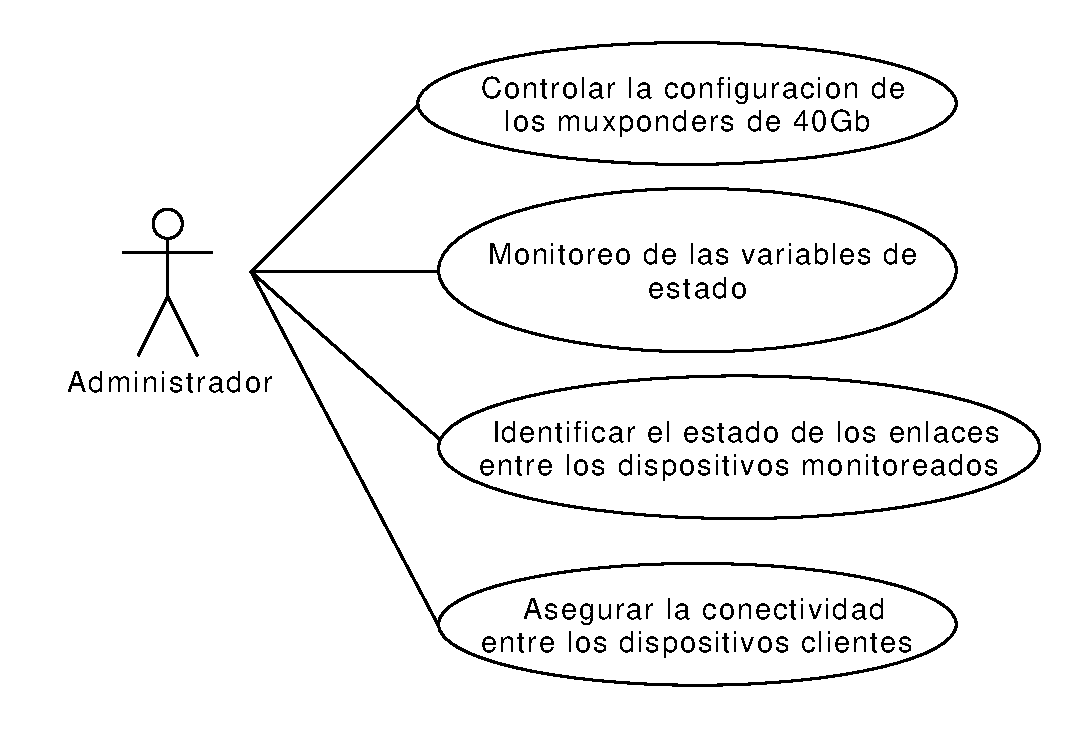
\includegraphics[scale=0.53]{Figures/caso_uso_admin.pdf}
  \caption{Probabilidad de ocurrencia del riesgo.}
  \label{fig:probabilidad_riesgo}
\end{figure}

Mientras que la figura \ref{fig:efectos_riesgo} describe el criterio que se utilizó para definir el impacto de los efectos del riesgo. 

\begin{figure}[H]
  \centering
  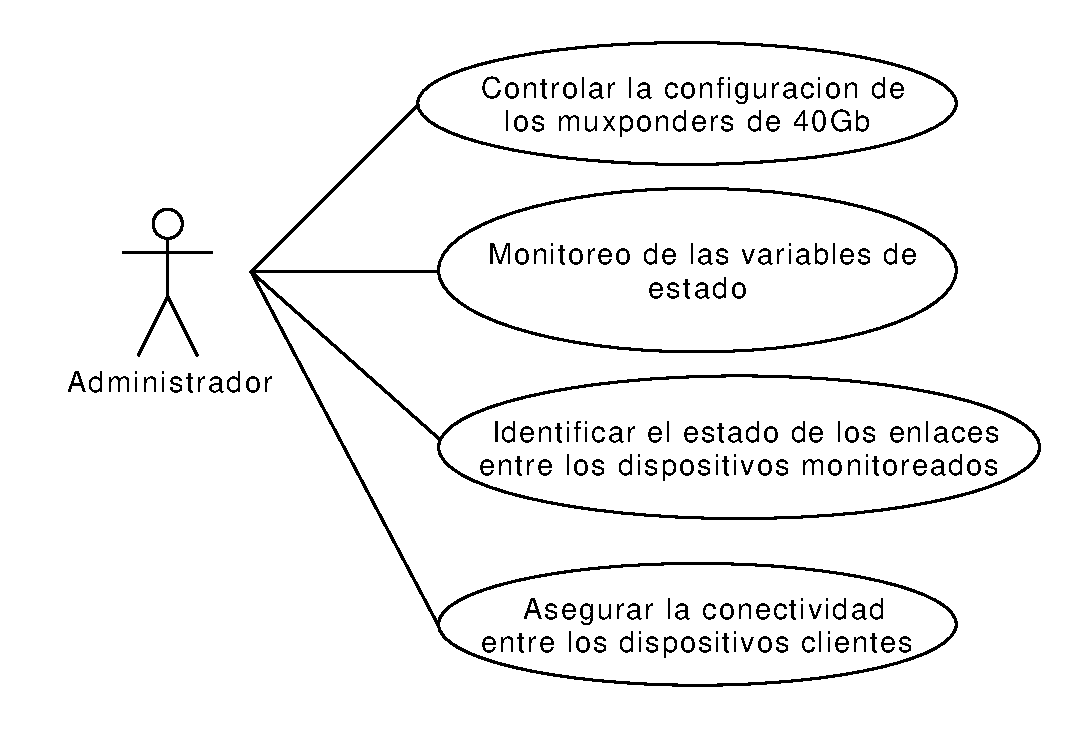
\includegraphics[scale=0.53]{Figures/caso_uso_admin.pdf}
  \caption{Impacto de los efectos del riesgo.}
  \label{fig:efectos_riesgo}
\end{figure}

Al combinar la probabilidad de aparición y los efectos del riesgo, se obtiene un nivel de exposición del riesgo. Esta última se puede ver de forma gráfica en la figura \ref{fig:niveles_riesgo}. 

\begin{figure}[H]
  \centering
  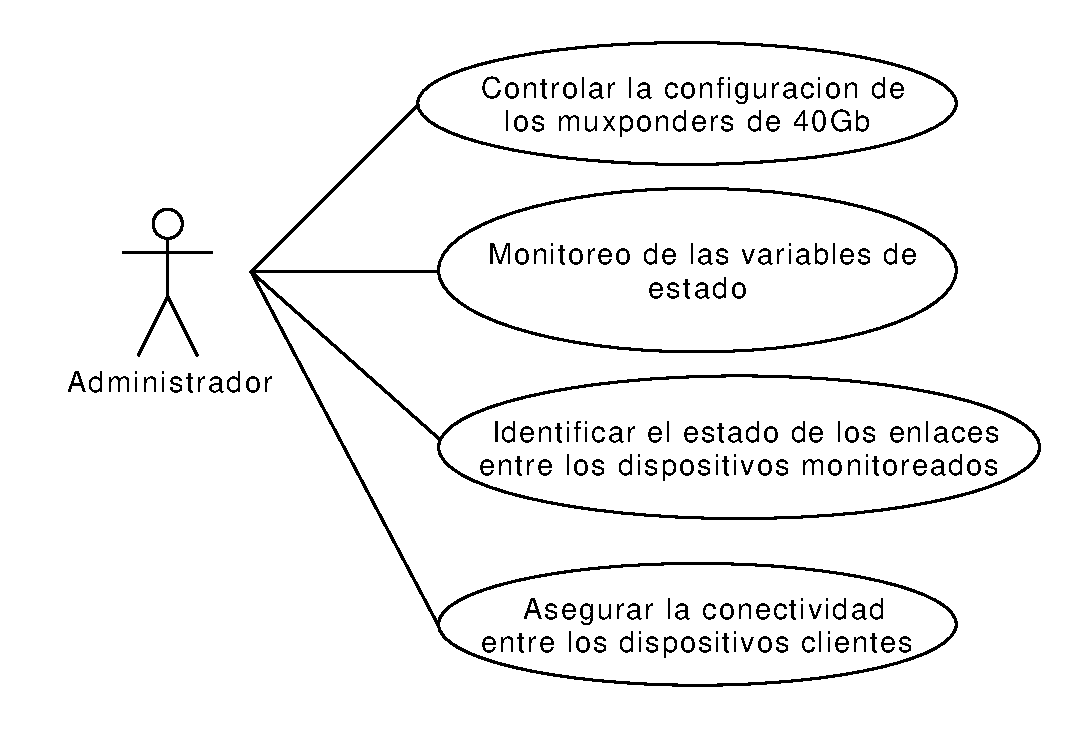
\includegraphics[scale=0.53]{Figures/caso_uso_admin.pdf}
  \caption{Impacto de los efectos del riesgo.}
  \label{fig:niveles_riesgo}
\end{figure}

Por otra parte, la figura \ref{fig:expo_riesgo} es utilizada como referencia para interpretar la exposición del riesgo.

\begin{figure}[H]
  \centering
  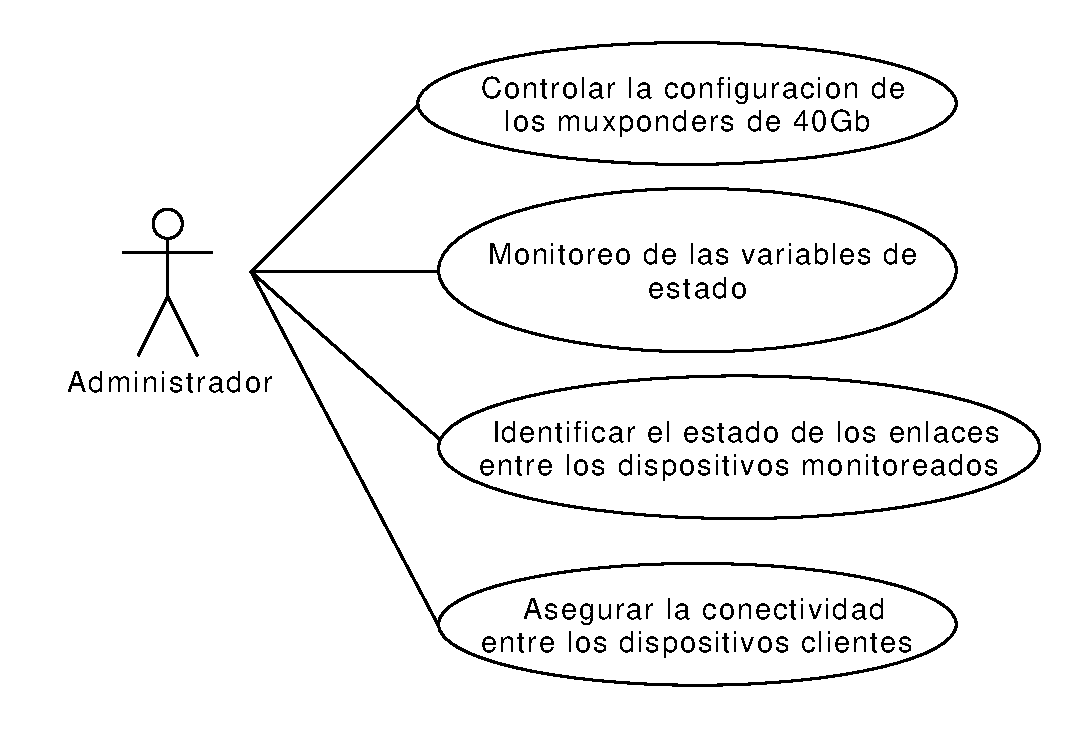
\includegraphics[scale=0.53]{Figures/caso_uso_admin.pdf}
  \caption{Referencia exposición del riesgo.}
  \label{fig:expo_riesgo}
\end{figure}